\chapter{Diseño e Implementación} % Main chapter title

\label{Chapter3} % Change X to a consecutive number; for referencing this chapter elsewhere, use \ref{ChapterX}

\definecolor{mygreen}{rgb}{0,0.6,0}
\definecolor{mygray}{rgb}{0.5,0.5,0.5}
\definecolor{mymauve}{rgb}{0.58,0,0.82}

%%%%%%%%%%%%%%%%%%%%%%%%%%%%%%%%%%%%%%%%%%%%%%%%%%%%%%%%%%%%%%%%%%%%%%%%%%%%%
% parámetros para configurar el formato del código en los entornos lstlisting
%%%%%%%%%%%%%%%%%%%%%%%%%%%%%%%%%%%%%%%%%%%%%%%%%%%%%%%%%%%%%%%%%%%%%%%%%%%%%
\lstset{ %
  backgroundcolor=\color{white},   % choose the background color; you must add \usepackage{color} or \usepackage{xcolor}
  basicstyle=\footnotesize,        % the size of the fonts that are used for the code
  breakatwhitespace=false,         % sets if automatic breaks should only happen at whitespace
  breaklines=true,                 % sets automatic line breaking
  captionpos=b,                    % sets the caption-position to bottom
  commentstyle=\color{mygreen},    % comment style
  deletekeywords={...},            % if you want to delete keywords from the given language
  %escapeinside={\%*}{*)},          % if you want to add LaTeX within your code
  %extendedchars=true,              % lets you use non-ASCII characters; for 8-bits encodings only, does not work with UTF-8
  %frame=single,	                % adds a frame around the code
  keepspaces=true,                 % keeps spaces in text, useful for keeping indentation of code (possibly needs columns=flexible)
  keywordstyle=\color{blue},       % keyword style
  language=[ANSI]C,                % the language of the code
  %otherkeywords={*,...},           % if you want to add more keywords to the set
  numbers=left,                    % where to put the line-numbers; possible values are (none, left, right)
  numbersep=5pt,                   % how far the line-numbers are from the code
  numberstyle=\tiny\color{mygray}, % the style that is used for the line-numbers
  rulecolor=\color{black},         % if not set, the frame-color may be changed on line-breaks within not-black text (e.g. comments (green here))
  showspaces=false,                % show spaces everywhere adding particular underscores; it overrides 'showstringspaces'
  showstringspaces=false,          % underline spaces within strings only
  showtabs=false,                  % show tabs within strings adding particular underscores
  stepnumber=1,                    % the step between two line-numbers. If it's 1, each line will be numbered
  stringstyle=\color{mymauve},     % string literal style
  tabsize=2,	                   % sets default tabsize to 2 spaces
  title=\lstname,                  % show the filename of files included with \lstinputlisting; also try caption instead of title
  morecomment=[s]{/*}{*/}
}


%----------------------------------------------------------------------------------------
%	SECTION 1
%----------------------------------------------------------------------------------------
%\section{Análisis del software}
% 
%La idea de esta sección es resaltar los problemas encontrados, los criterios utilizados y la justificación de las decisiones que se hayan tomado.
%
%Se puede agregar código o pseudocódigo dentro de un entorno lstlisting con el siguiente código:
%
%\begin{verbatim}
%\begin{lstlisting}[caption= "un epígrafe descriptivo"]
%	las líneas de código irían aquí...
%\end{lstlisting}
%\end{verbatim}
%
%A modo de ejemplo:
%
%\begin{lstlisting}[label=cod:vControl,caption=Pseudocódigo del lazo principal de control.]  % Start your code-block
%
%#define MAX_SENSOR_NUMBER 3
%#define MAX_ALARM_NUMBER  6
%#define MAX_ACTUATOR_NUMBER 6
%
%uint32_t sensorValue[MAX_SENSOR_NUMBER];		
%FunctionalState alarmControl[MAX_ALARM_NUMBER];	//ENABLE or DISABLE
%state_t alarmState[MAX_ALARM_NUMBER];						//ON or OFF
%state_t actuatorState[MAX_ACTUATOR_NUMBER];			//ON or OFF
%
%void vControl() {
%
%	initGlobalVariables();
%	
%	period = 500 ms;
%		
%	while(1) {
%
%		ticks = xTaskGetTickCount();
%		
%		updateSensors();
%		
%		updateAlarms();
%		
%		controlActuators();
%		
%		vTaskDelayUntil(&ticks, period);
%	}
%}
%\end{lstlisting}

%Es este capítulo se presentarán las topologías básicas del sistema ferroviario y los dos enfoques de resolución del proyecto, con sus ventajas y desventajas antes de abordar la implementación de la solución elegida.

En este capítulo se presentarán las decisiones de diseño adoptadas para concretar el desarrollo del trabajo. Además de describir en forma genérica los módulos necesarios tanto del sistema de enclavamiento como de los bloques auxiliares para concretar una comunicación exitosa entre el sistema y el exterior.


\section{Consideraciones generales}

En el presente trabajo se optó por implementar el sistema bajo el enfoque funcional. Asumiendo que sus ventajas son mucho mas fuertes que sus desventajas y el análisis de los resultados obtenidos fueron mucho mas provechosos que los de su contraparte funcional.

Los módulos del sistema fueron implementados con máquinas de estado finitas con camino de datos (FSMD, del inglés \textit{Finite State Machine with Data path}), que son máquinas de estado finitas (FSM, del inglés \textit{Finite State Machine}) y circuitos secuenciales. La FSMD (Figura \ref{fig:FSMD}) posee dos partes diferenciadas: el camino de control y el camino de datos. El camino de control contiene una FSM que ,según las entradas de control y el estado interno que posee, genera señales de control internas que controlan los circuitos secuenciales del camino de datos que contienen los bloques que procesan las entradas y actúan sobre las salidas.

	\begin{figure}[h]
	\centering
		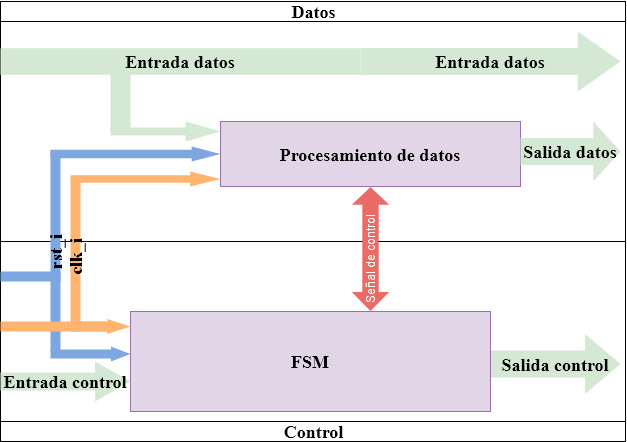
\includegraphics[scale=.5]{./Figures/FSMD}
		\caption{Diagrama en bloques genérico de una FSMD}
		\label{fig:FSMD}
	\end{figure}
	
	\vspace{5cm}
	
	Siguiendo los lineamientos recomendados, una FSMD debe ser diseñada, implementada y simulada siguiendo los siguientes pasos:
	
	\begin{enumerate}
		\item Definición del algoritmo a implementar.
		\item Definición de entradas y salidas de la FSMD.
		\item Diseño del camino de datos.
		\item Diseño de interfaz entre camino de datos y camino de control.
		\item Definición de los estados de la FSM.
		\item Diseño de la FSM.
		\item Implementar el diseño.
		\item Diseñar e implementar los ensayos.
	\end{enumerate}
	
	Esta metodología puede inferir mas tiempo de desarrollo que el habitual, pero ya ha demostrado ser exitosa en el proyecto realizado por el Mg. Ing. Facundo Larosa, codirector de este trabajo. Por lo que se aprovechó su experiencia y conocimiento para resolver esta etapa del desarrollo. Los beneficios son un mayor control del diseño a bajo nivel, una mayor portabilidad y un mas eficiente uso de los recursos de la plataforma electrónica.

\section{Análisis de la red ferroviaria y generación automática del código}

	Todo grafo ferroviario necesita dos datos para estar definido. El primero es la una lista de relaciones entre nodo inicial y nodo final, el segundo es la posición absoluta del nodo en el grafo junto con datos adicionales como si posee un paso a nivel o si es bidireccional. Con esa información es posible realizar un análisis para obtener un resultado como el que se presenta en la Figura \ref{fig:Mapa} al ingresar un grafo de una red ferroviaria bypass.	

	\begin{figure}[h]
	\centering
		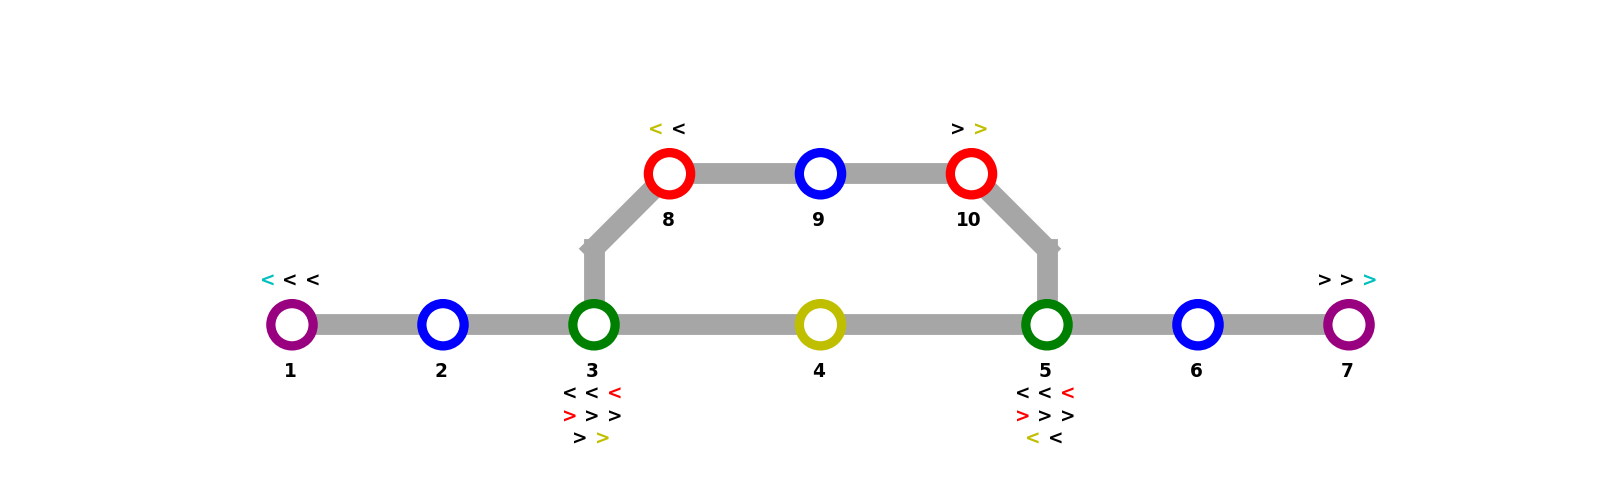
\includegraphics[scale=.4]{./Figures/Mapa_2}
		\caption{Grafo luego de ser analizado por el algoritmo}
		\label{fig:Mapa}
	\end{figure}

	Los nodos 1 y 7 se encuentran pintados de violeta porque al tener un único vecino cada uno se consideran nodos extremos. Los nodos 2,6 y 9 no presentan nada en especial por lo que son nodos simples. Los que si tienen una importancia central en el análisis son los nodos que poseen tres vecinos: el nodo 3 y el nodo 5, que son pintados en verde y se consideran cambios raíz.

	Luego el nodo 4 es categoriza como nodo cambio directo por ser la continuación de los segmentos 2-3 y 5-6 de tener el cambio de vía en posición normal, permitiendo la circulación directa. En este caso el nodo 4 es compartido por ambos cambios pero no siempre se da este caso.
	
	Los nodos 8 y 10, siendo vecinos de los cambios 3 y 5 pero no compartiendo ninguna coordenada espacial con ellos, son nodos de cambios ramificados. Es decir, solo permitirán la secuencia de nodos 2-3-8 o 9-8-3 si la máquina de cambios se encuentra en posición inversa. Para el nodo 5 el análisis es análogo.

	La asignación de semáforos se realiza solo sobre los nodos extremos, cambios raíz y cambios ramificados. Los extremos necesitan los semáforos para permitir la salida de las formaciones de la red, ya que la red ferroviaria continua mas allá del nodo 1 y del 7, de ser nodos extremos absolutos (fin de red) no corresponde que se les asigne un semáforo.
	
	Los nodos de cambios son los que presentan mayor cantidad de semáforos. Necesitan dos semáforos de tres aspectos para permitir la circulación directa sobre el cambio cuando se encuentra en posición normal y un semáforo de dos aspectos para permitir la circulación en la ramificación del recorrido, pero con precaución por ser una zona crítica. Finalmente los nodos de cambios ramificados solo presentan un semáforo de doble aspectos como complemento al otro semáforo de maniobras, para permitir utilizar la ramificación para volver al recorrido principal a una velocidad moderada. 

\section{Módulo de nodos}

	\begin{figure}[h]
	\centering
	%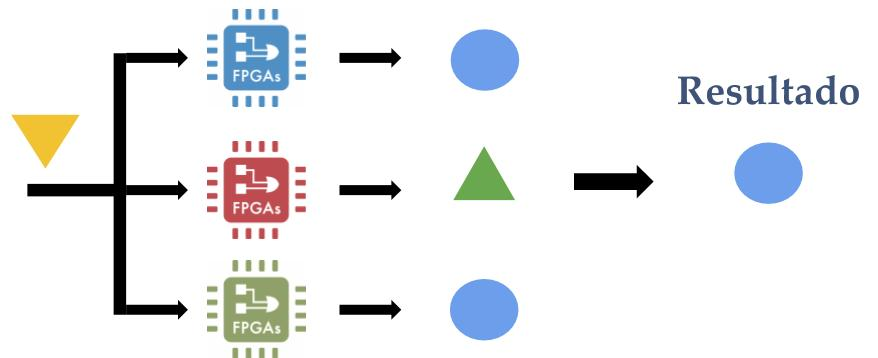
\includegraphics[scale=.3]{./Figures/Redundancia}
		\caption{HOLA}
		\label{fig:hola}
	\end{figure}
	\improvement{Incluir figura}	
	
\section{Módulo de cambios}

	\begin{figure}[h]
	\centering
	%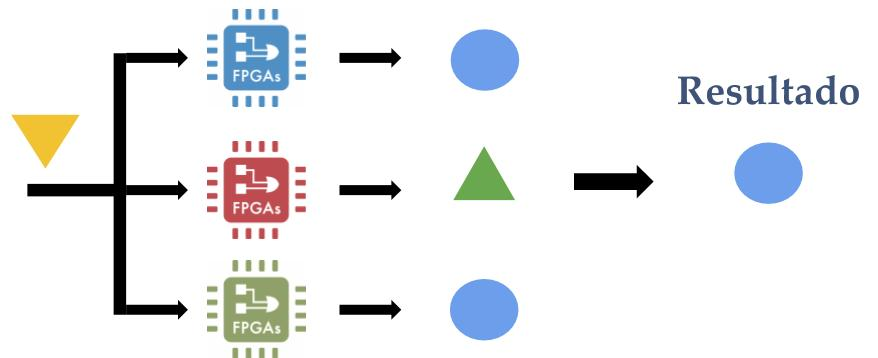
\includegraphics[scale=.3]{./Figures/Redundancia}
		\caption{HOLA}
		\label{fig:hola}
	\end{figure}
	\improvement{Incluir figura}	
	
\section{Módulo de red}

	\begin{figure}[h]
	\centering
	%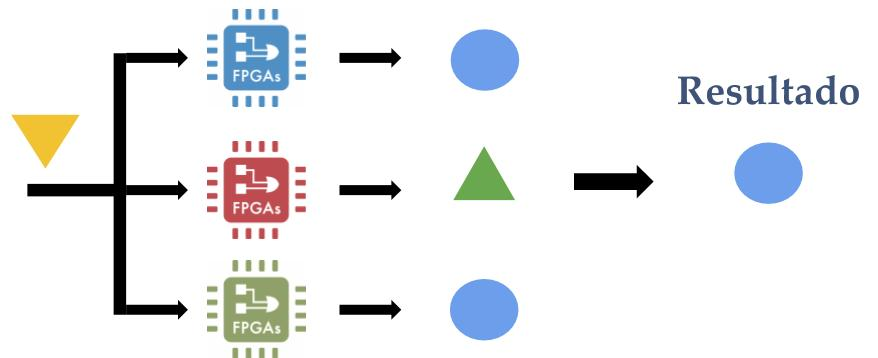
\includegraphics[scale=.3]{./Figures/Redundancia}
		\caption{HOLA}
		\label{fig:hola}
	\end{figure}
	\improvement{Incluir figura}	
	
\section{Módulos de adaptación a enclavamiento}

	Explicacion Explicacion Explicacion Explicacion Explicacion Explicacion Explicacion Explicacion Explicacion Explicacion Explicacion Explicacion Explicacion Explicacion Explicacion Explicacion Explicacion Explicacion Explicacion Explicacion Explicacion Explicacion Explicacion Explicacion Explicacion Explicacion Explicacion Explicacion Explicacion Explicacion Explicacion Explicacion Explicacion Explicacion 
	 
	\subsection{Módulo separador}
	
		Explicacion Explicacion Explicacion Explicacion Explicacion Explicacion Explicacion Explicacion Explicacion Explicacion Explicacion Explicacion Explicacion Explicacion Explicacion Explicacion Explicacion Explicacion Explicacion Explicacion Explicacion Explicacion Explicacion Explicacion Explicacion Explicacion Explicacion Explicacion Explicacion Explicacion 
		
		\begin{figure}[h]
		\centering
			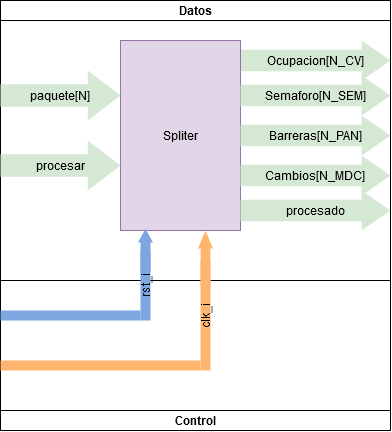
\includegraphics[scale=.5]{./Figures/FSMD-Separador}
			\caption{FSMD del módulo separador}
			\label{fig:FSMD_Separador}
		\end{figure}
		
		Explicacion Explicacion Explicacion Explicacion Explicacion Explicacion Explicacion Explicacion Explicacion Explicacion Explicacion Explicacion Explicacion Explicacion Explicacion Explicacion Explicacion Explicacion Explicacion Explicacion Explicacion Explicacion Explicacion Explicacion Explicacion Explicacion Explicacion Explicacion Explicacion Explicacion 
		
	\subsection{Módulo mediador}
	
		Explicacion Explicacion Explicacion Explicacion Explicacion Explicacion Explicacion Explicacion Explicacion Explicacion Explicacion Explicacion Explicacion Explicacion Explicacion Explicacion Explicacion Explicacion Explicacion Explicacion Explicacion Explicacion Explicacion Explicacion Explicacion Explicacion Explicacion Explicacion Explicacion Explicacion Explicacion Explicacion Explicacion Explicacion 
		
		\begin{figure}[h]
		\centering
			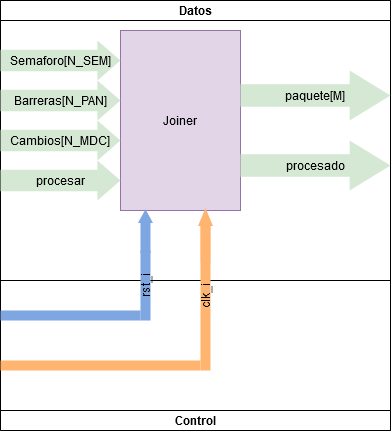
\includegraphics[scale=.5]{./Figures/FSMD-Mediador}
			\caption{FSMD del módulo mediador}
			\label{fig:FSMD_Mediador}
		\end{figure}
		
		Explicacion Explicacion Explicacion Explicacion Explicacion Explicacion Explicacion Explicacion Explicacion Explicacion Explicacion Explicacion Explicacion Explicacion Explicacion Explicacion Explicacion Explicacion Explicacion Explicacion Explicacion Explicacion Explicacion Explicacion Explicacion Explicacion Explicacion Explicacion 
		
\section{Módulos de procesamiento de tramas}

	Explicacion Explicacion Explicacion Explicacion Explicacion Explicacion Explicacion Explicacion Explicacion Explicacion Explicacion Explicacion Explicacion Explicacion Explicacion Explicacion Explicacion Explicacion Explicacion Explicacion Explicacion Explicacion Explicacion Explicacion Explicacion Explicacion Explicacion Explicacion Explicacion 
	
	\subsection{Módulo detector}
	
		Explicacion Explicacion Explicacion Explicacion Explicacion Explicacion Explicacion Explicacion Explicacion Explicacion Explicacion Explicacion Explicacion Explicacion Explicacion Explicacion Explicacion Explicacion Explicacion Explicacion Explicacion Explicacion Explicacion Explicacion Explicacion Explicacion Explicacion Explicacion Explicacion Explicacion Explicacion 
		
		\begin{figure}[h]
		\centering
			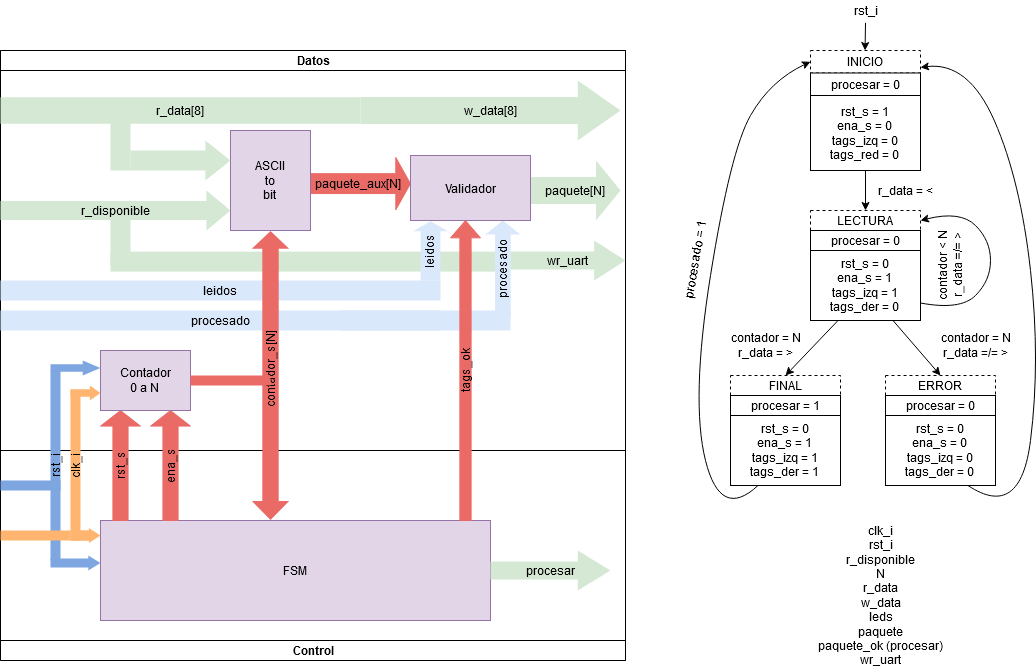
\includegraphics[scale=.4]{./Figures/FSMD-Detector}
			\caption{FSMD del módulo detector}
			\label{fig:FSMD_Detector}
		\end{figure}
		
		Explicacion Explicacion Explicacion Explicacion Explicacion Explicacion Explicacion Explicacion Explicacion Explicacion Explicacion Explicacion Explicacion Explicacion Explicacion Explicacion Explicacion Explicacion Explicacion Explicacion Explicacion Explicacion Explicacion Explicacion Explicacion Explicacion Explicacion Explicacion 
		
	\subsection{Módulo registro}
	
		Explicacion Explicacion Explicacion Explicacion Explicacion Explicacion Explicacion Explicacion Explicacion Explicacion Explicacion Explicacion Explicacion Explicacion Explicacion 
		
		\begin{figure}[h]
		\centering
			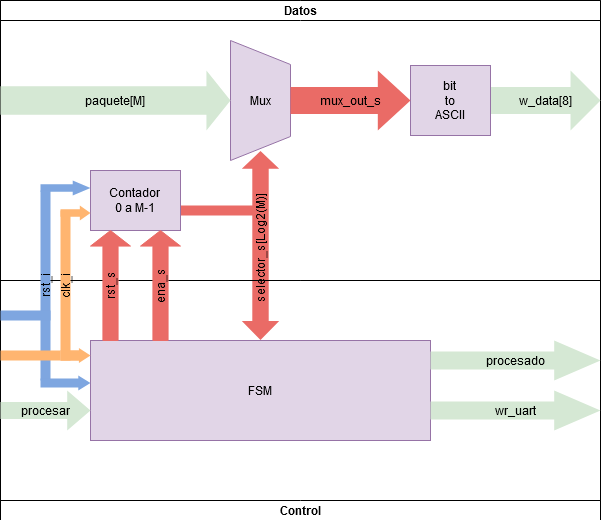
\includegraphics[scale=.4]{./Figures/FSMD-Registro}
			\caption{FSMD del módulo registro}
			\label{fig:FSMD_Registro}
		\end{figure}

		Explicacion Explicacion Explicacion Explicacion Explicacion Explicacion Explicacion Explicacion Explicacion Explicacion Explicacion Explicacion Explicacion Explicacion Explicacion Explicacion Explicacion Explicacion Explicacion Explicacion Explicacion 
		
	\subsection{Módulo selector}
	
		Explicacion 
		
		\begin{figure}[h]
		\centering
			%\includegraphics[scale=.3]{./Figures/FSMD_Selector}
			\caption{Diagrama de estados finitos digitales del módulo selector}
			\label{fig:FSMD_Selector}
		\end{figure}
		\improvement{Incluir figura}	
		
		Explicacion 
		
\section{Módulo de comunicación UART}

		\begin{figure}[h]
		\centering
		%\includegraphics[scale=.3]{./Figures/FSMD_UART}
			\caption{Diagrama de estados finitos digitales del módulo UART}
			\label{fig:FSMD_UART}
		\end{figure}
		\improvement{Incluir figura}

\section{Interfaz de comunicación Python}

		\begin{figure}[h]
		\centering
		%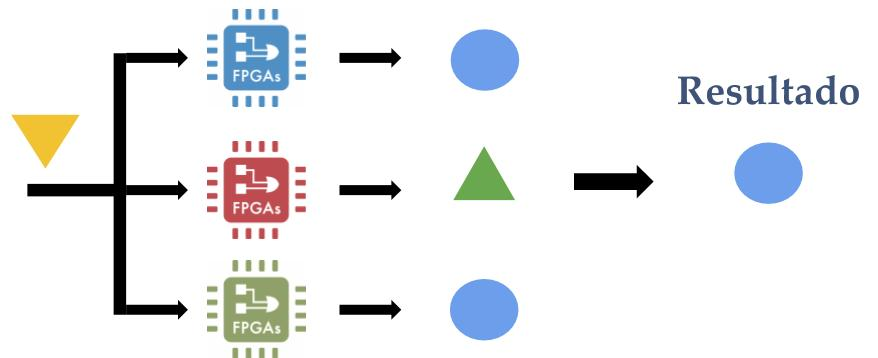
\includegraphics[scale=.3]{./Figures/Redundancia}
			\caption{HOLA}
			\label{fig:hola}
		\end{figure}
		\improvement{Incluir figura}